\section{Overview}
\label{sec:overview}

% You may need to move this \begin{figure} ... \end{figure} block around
% in the document to place it in a logical spot in the paper. In
% general, get the figure on the same page as the prose that refers to
% it.
\begin{figure}[t]
  \centering
  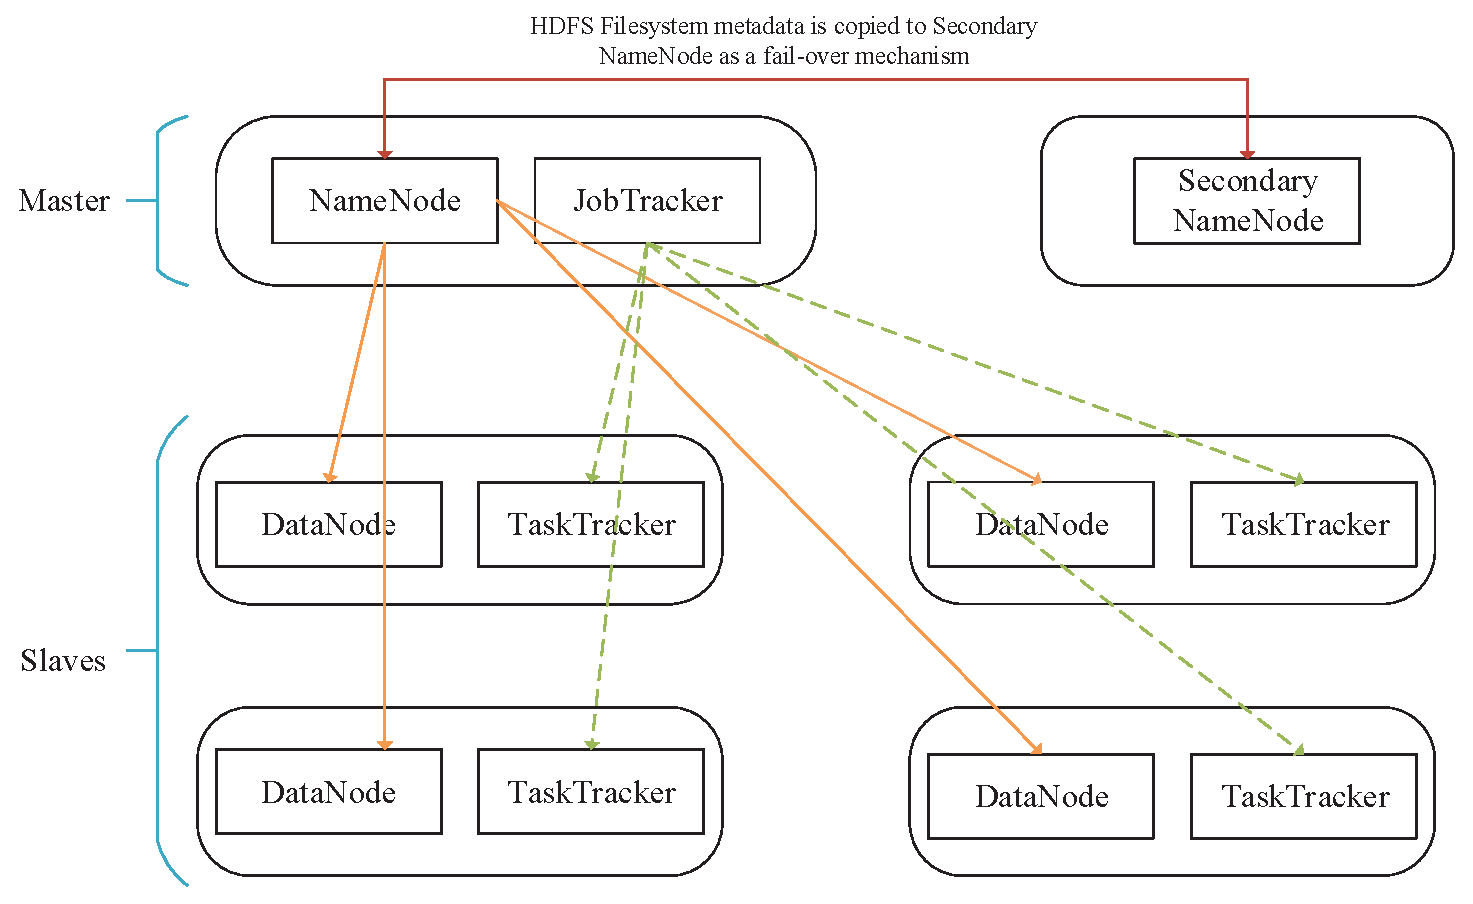
\includegraphics[width=3in]{figs/HadoopOverview.eps}
  \caption{Hadoop Overview}
  \label{fig:overview}
\end{figure}

This section presents details about Hadoop and Docker.

\subsection{Hadoop}

Hadoop is a large-scale data processing framework that is designed to scale up from a single server to thousands of machines, with very high degree of fault tolerance. Rather than relying on high-end hardware, the resiliency of these clusters comes from the software's ability to detect and handle failures at the application layer.

HDFS(storage) and MapReduce~\cite{dean2008mapreduce} (processing) are the two core components of Hadoop. The most important aspect of Hadoop is that both HDFS and MapReduce are designed with each other in mind and each are co-deployed such that there is a single cluster and thus provides the ability to move computation to the data not the other way around. Thus, the storage system is not physically separate from a processing system.

The main components of HDFS are NameNode, DataNodes, and Secondary NameNode. NameNode is the master of the system. It maintains the name system (directories and files) and manages the blocks which are present on the DataNodes. DataNodes are the slaves which are deployed on each machine and provide the actual storage. Secondary NameNode is responsible for performing periodic checkpoints. Notice that Secondary NameNode is not a back up server of Namenode.

The main components of MapReduce are JobTracker and Tasktracker. JobTracker is the master of the system which manages the jobs and resources in the cluster (TaskTrackers).  TaskTrackers are the slaves which are deployed on each machine. They are responsible for running the map and reduce tasks as instructed by the JobTracker.

However, Hadoop 1.x  is not scalable enough and has many limitations. There is no horizontal scalability of NameNode and it does not support NameNode High Availability. It can only support up to 4,000 nodes per cluster. Map and Reduce task slots are static. The JobTracker is responsible for both resource management and job scheduling, so it is so overburdened that it becomes the bottleneck of Hadoop.Therefore, Hadoop 2.x or Hadoop YARN is developed to handle the scalability problem in Hadoop. The fundamental idea of Haoop 2.x is to split up the two major functionalities of the JobTracker, resource management and job scheduling, into separate daemons. The following figure shows the architecture of Hadoop 2.x.

\begin{figure}[t]
  \centering
  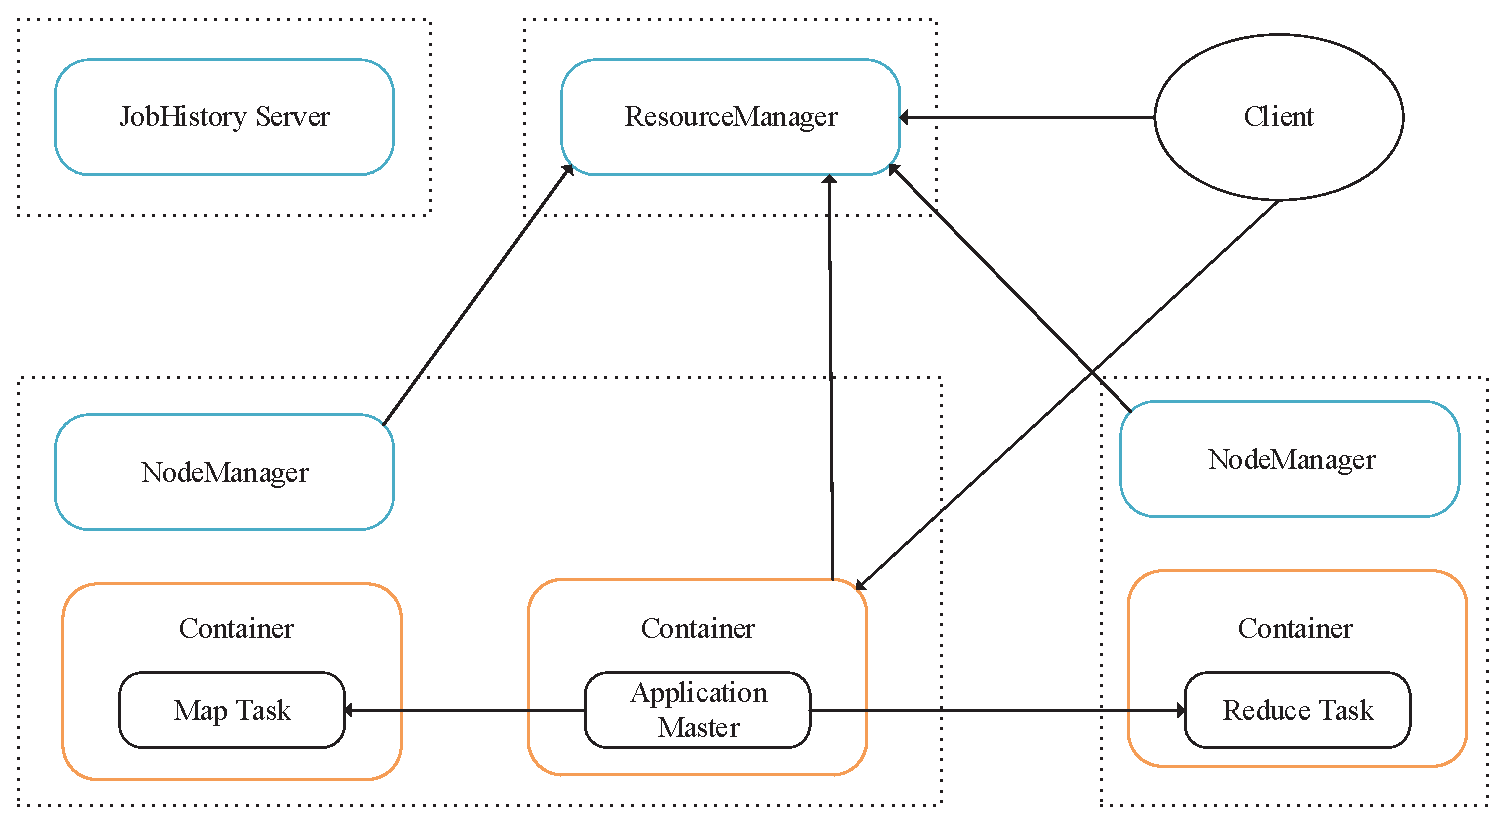
\includegraphics[width=3in]{figs/Container.eps}
  \caption{Hadoop Container}
  \label{fig:overview}
\end{figure}


\begin{figure}[t]
  \centering
  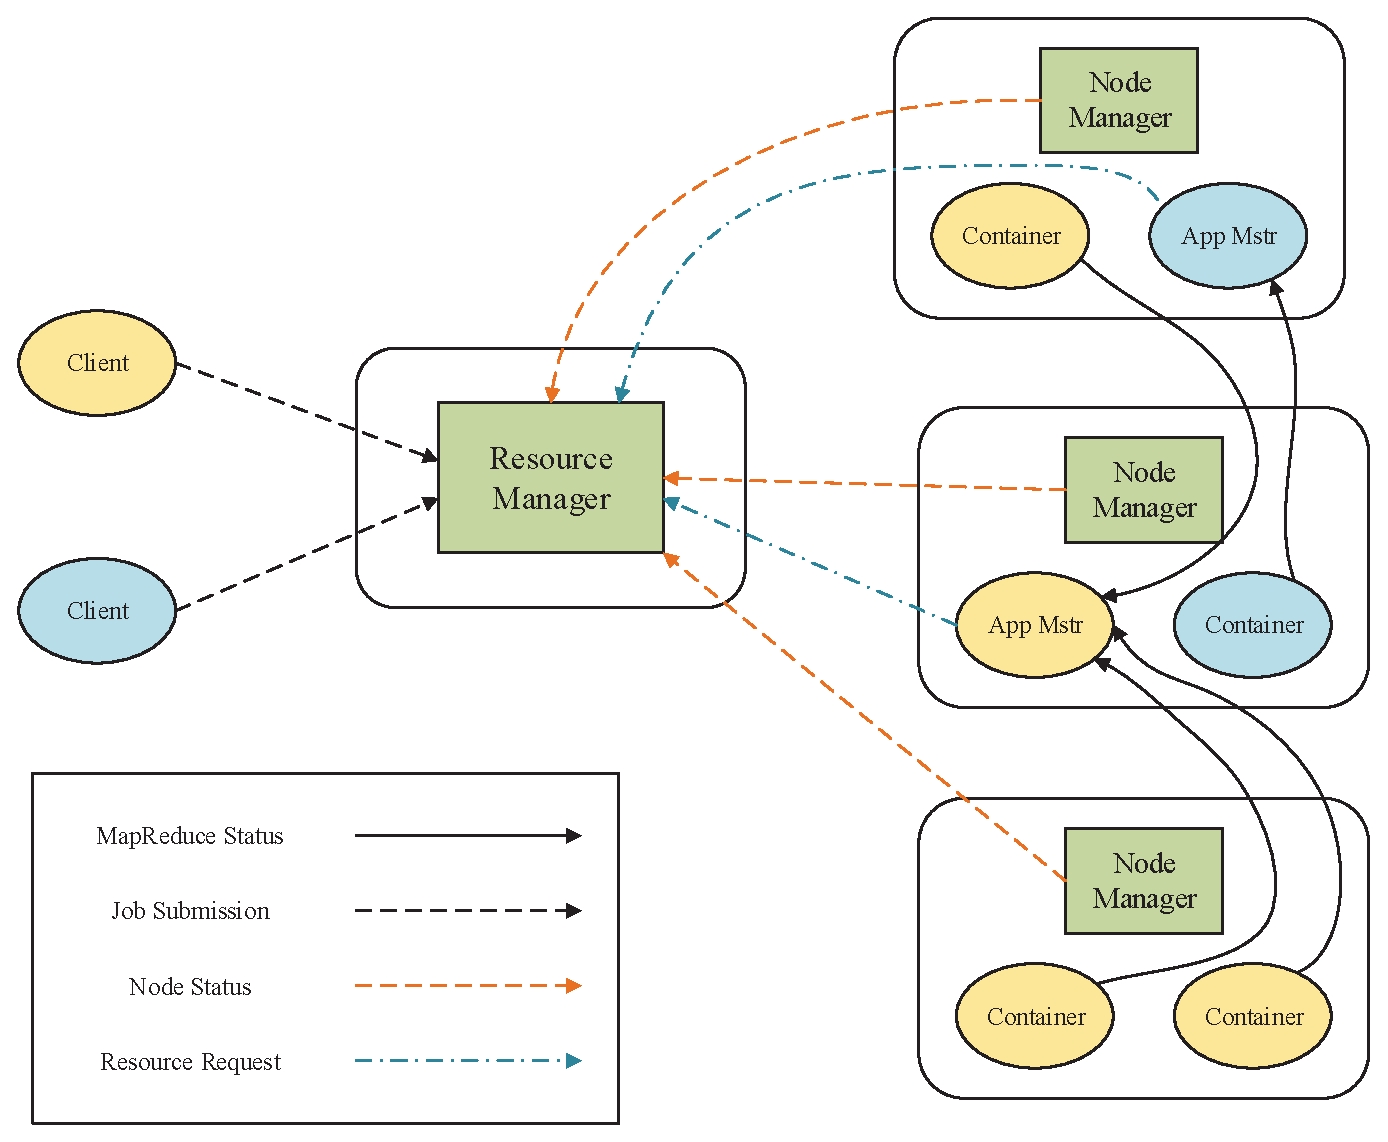
\includegraphics[width=3in]{figs/yarn.eps}
  \caption{Yarn Architecture}
  \label{fig:overview}
\end{figure}


HDFS does not change in Hadoop 2.x. The YARN component is introduced to replace JobTracker. It has three components: Resource Manager,Node Manager, and Application Master. ResourceManager is the master that arbitrates all the available cluster resources and thus helps manage the distributed applications running on the YARN system. The NodeManager is YARN’s per-node agent, and takes care of the individual compute nodes in a Hadoop cluster, such as keeping up-to date with the ResourceManager, overseeing containers’ life-cycle management; monitoring resource usage (memory, CPU) of individual containers, etc. The ApplicationMaster is, in effect, an instance of a framework-specific library and is responsible for negotiating resources from the ResourceManager and working with the NodeManager(s) to execute and monitor the containers and their resource consumption. It has the responsibility of negotiating appropriate resource containers from the ResourceManager, tracking their status and monitoring progress.

\subsection{Docker in Hadoop}
Docker is an open platform for developing, shipping, and running applications. It is a Linux-based system that makes use of LXC~\cite{helsley2009lxc} that automates the deployment of applications inside software containers, by providing an additional layer of abstraction and automation of operating system level virtualization on Linux. Docker uses resource isolation features of the Linux kernel such as cgroups, and kernel namespace to allow independent "containers" to run within a single Linux instance, avoiding the overhead of starting virtual machines. With Docker we can separate our applications form the infrastructure and treat the infrastructure like a managed application. 

As we can see from the Figure 3, the Docker Engine Container compromises just the application and its dependencies. It provides a way to run almost any application securely isolated in a container. It runs as an isolated process in userspace on the host operating system, sharing the kernel with other containers, so that many containers are allowed to run simultaneously on the host. The lightweight nature of containers, which run without extra load of a hypervisor, means it enjoys the resource isolation and allocation benefits of virtual machines but is much more portable and efficient.

\begin{figure}[t]
  \centering
  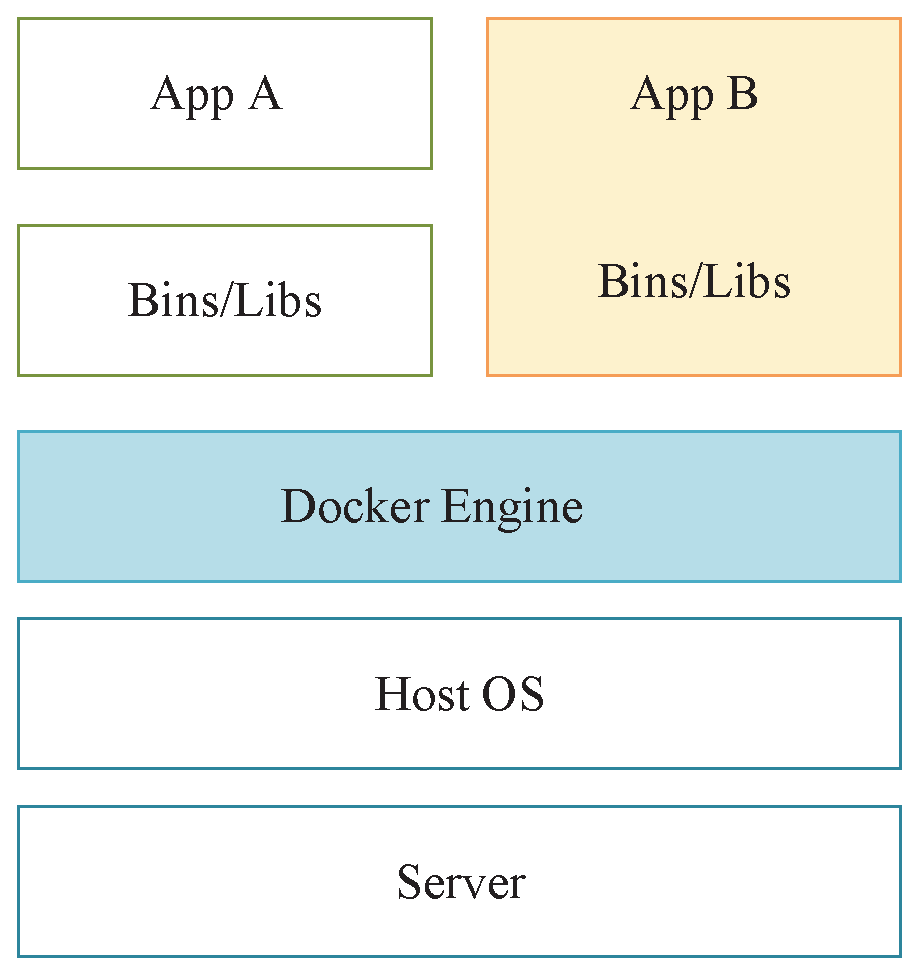
\includegraphics[width=2in]{figs/docker.eps}
  \caption{Docker}
  \label{fig:overview}
\end{figure}

Hadoop YARN container represents a collection of physical resources, including CPU cores, disk along with RAM. Docker container can perfectly implement this concept. By using Docker containers, resources can be isolated, services restricted, and processes provisioned to have a private view of the operating system with their own process ID space, file system structure, and network interfaces. Docker Container Executor (DCE) is thus developed. Other container executors are Default Container Executor and Linux Container Executor which is implemented with cgroups.

